
\documentclass[letterpaper, 10 pt, conference]{ieeeconf}

\IEEEoverridecommandlockouts                              % This command is only needed if 
   % you want to use the \thanks command

\overrideIEEEmargins    
\usepackage{graphicx}
\usepackage{tabu}
\usepackage{amsmath,amssymb}
\usepackage{algorithm}
\usepackage[noend]{algpseudocode}
\usepackage{longtable}
\usepackage{mathtools}
\usepackage{breqn}
\usepackage{amsmath}
\DeclareMathOperator*{\argmax}{arg\,max}
\DeclareMathOperator*{\argmin}{arg\,min}


%\documentclass{article}

% Needed to meet printer requirements.

% See the \addtolength command later in the file to balance the column lengths
% on the last page of the document

% The following packages can be found on http:\\www.ctan.org
%\usepackage{graphics} % for pdf, bitmapped graphics files
%\usepackage{epsfig} % for postscript graphics files
%\usepackage{mathptmx} % assumes new font selection scheme installed
%\usepackage{times} % assumes new font selection scheme installed
%\usepackage{amsmath} % assumes amsmath package installed
%\usepackage{amssymb}  % assumes amsmath package installed




\title{\LARGE \bf
Switched Soft Actor Critic \\
For The Acrobot Swing-up And Balance Task
}
\author{Sean Gillen, Marco Molnar, and Katie Byl% <-this % stops a space
\thanks{*This work was funded in part by NSF NRI award 1526424.}% <-this % stops a space
\thanks{Sean Gillen and Katie Byl are with the Electrical and Computer Engineering Department at the University of California, Santa Barbara CA 93106
{\tt\small sgillen@ucsb.edu},
{\tt\small katiebyl@ucsb.edu}.
Marco Molnar is with TU Berlin
{\tt\small marco.molnar@posteo.de}.}
        }

%\thanks{* Acknowledge a grant here}% <-this % stops a space
%\thanks{$^{1}$ UCSB}

\begin{document}

\DeclarePairedDelimiterX{\infdivx}[2]{(}{)}{%
  #1\;\delimsize\|\;#2%
}
\newcommand{\infdiv}{D\infdivx}
\DeclarePairedDelimiter{\norm}{\lVert}{\rVert}

\maketitle
%\thispagestyle{empty}
%\pagestyle{empty}



!!!! TODO

Clean up everything, especially algorithmic section
Do wahtever vis you are doing 
Clean up and upload code
address and remove all !!!s



%%%%%%%%%%%%%%%%%%%%%%%%%%%%%%%%%%%%%%%%%%%%%%%%%%%%%%%%%%%%%%%%%%%%%%%%%%%%%%%%
\begin{abstract}
In this work we present switched soft actor critic (SSAC), a novel extension of SAC that allows designers to combine traditional controllers with learned policies. This combination allows engineers to leverage both their own domain knowledge and the advantages of model free reinforcement learning. Unlike prior work, our method simultaneously learns neural network policies and the transitions between these policies. As a case study we apply our method to the Acrobot system, for this problem we combine a hand designed linear quadratic regulator (LQR) with a learned swing-up controller. We demonstrate that our technique outperforms other state of the art reinforcement learning algorithms in this setting. 
\end{abstract}


%%%%%%%%%%%%%%%%%%%%%%%%%%%%%%%%%%%%%%%%%%%%%%%%%%%%%%%%%%%%%%%%%%%%%%%%%%%%%%%%
\section{INTRODUCTION}

Advances in computing power and learning and stuff have allowed modern model free reinforcement learning to solve some really hard problems. Recent examples include controlling a 47 DOF humanoid to navigate a variety of obstacles \cite{heess_emergence_2017}, dexterously manipulating objects with a 24 DOF robotic hand, \cite{openai_learning_2018}, and controlling a physical quadruped robot run \cite{hwangbo_learning_2019}, and recover from falls \cite{lee_robust_2019}.

!!! add another paragraph talking about RL I think

Despite seeing success on very hard problems, these algorithms largely struggle on some low dimensional problems from the nonlinear control literature. Namely the acrobot \cite{spong_swing_1994} and the classic cart pole pendulum. These are both under-actuated mechanical systems that have unstable fixed points in their unforced dynamics (see section \ref{section:Acrobot} for specifics). The goal for the controller is to bring the system to this fixed point and keep it there. In this paper we focus on the acrobot as we found less examples of model free reinforcement learning performing well on this task.

\begin{figure}[ht]
\centering
  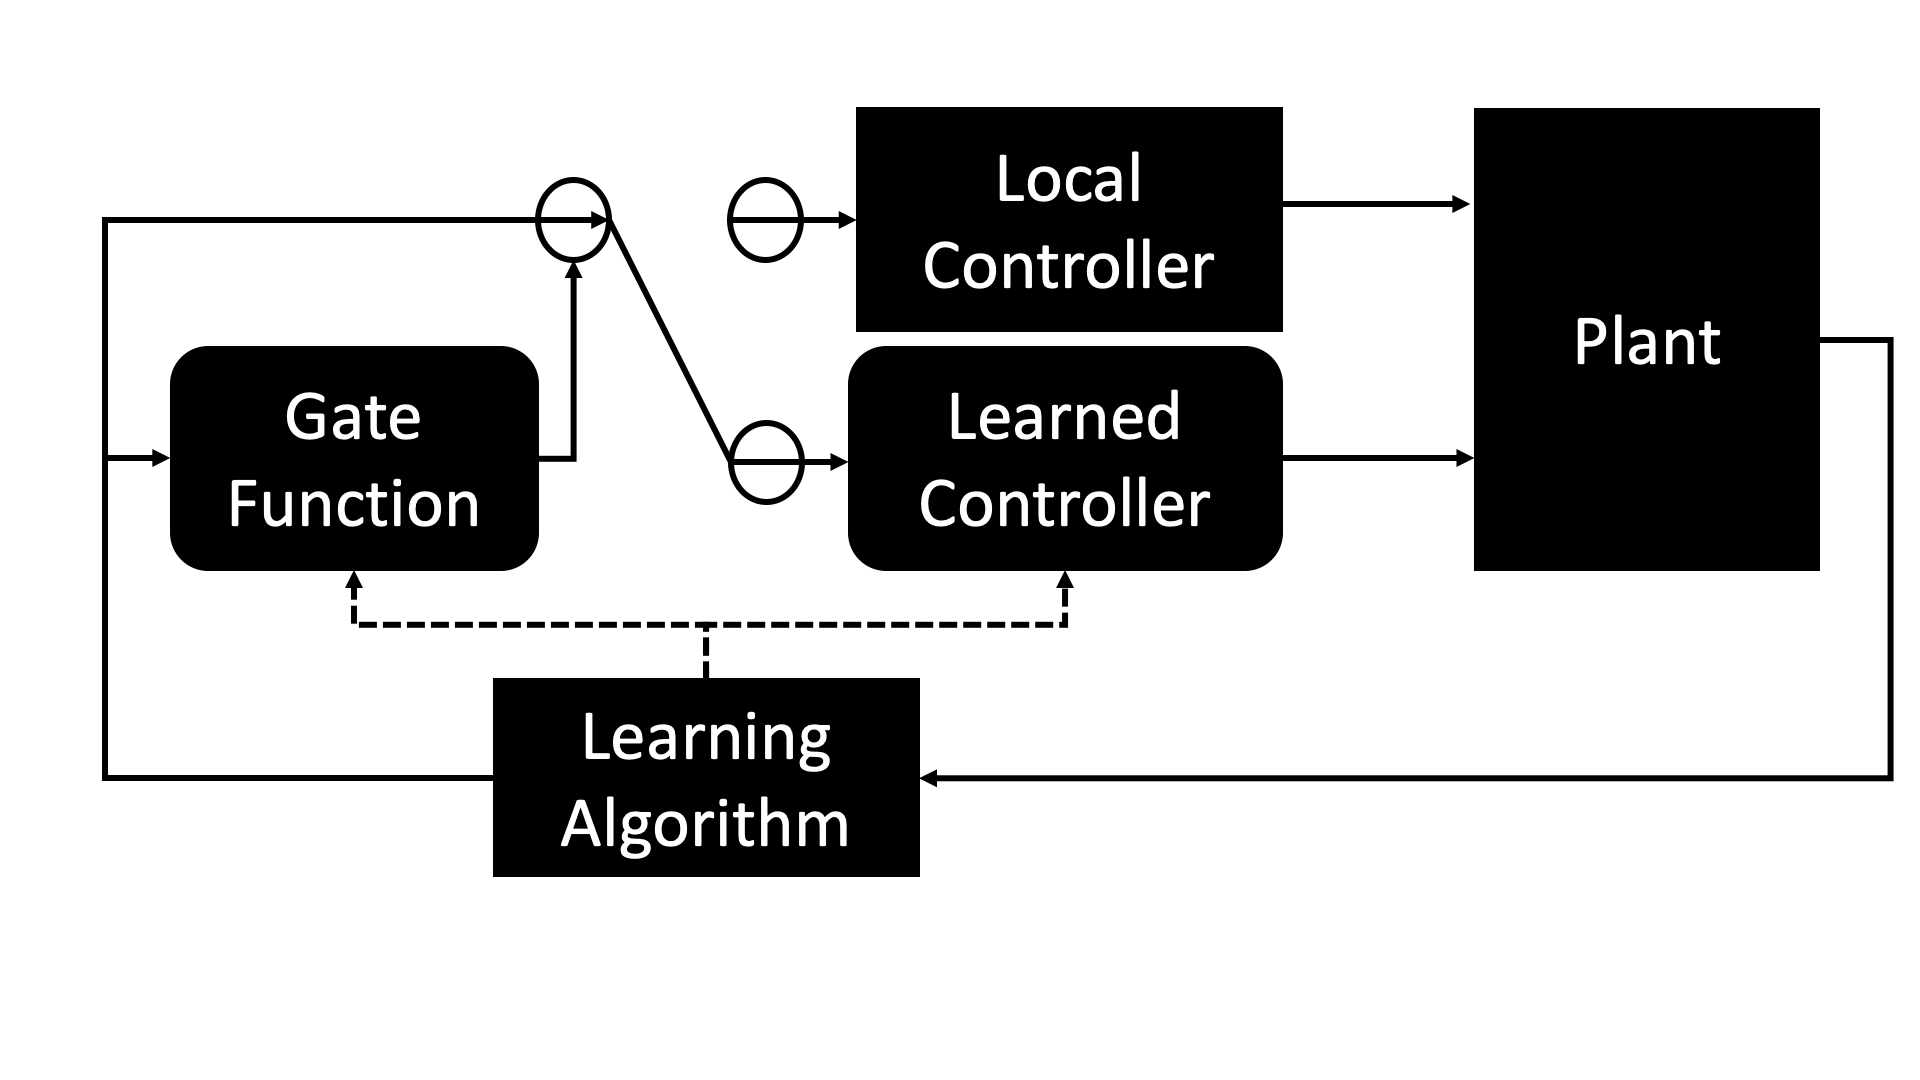
\includegraphics[scale=.25]{system5.png}
  \caption{System diagram for our technique. Rounded boxes represent learned neural networks, squared boxes represent static functions }
  \label{fig:hyst}
\end{figure}


It is not uncommon to see some variation of these systems tackled in various reinforcement benchmarks, but we have found these problems have usually been modified in a way to make them much easier. For example in the popular OpenAI Gym benchmarks \cite{1606.01540} the acrobot system is present, but the objective is only to get the system in the rough area of the unstable fixed point, and the dynamics are integrated with euler integration with a time-step of .2 seconds, which makes the problem much easier. We have modified this environment to include a higher order integrator with a smaller timestep, and changed the objective such that the system needs to be held at the unstable fixed point. We have found that almost universally, modern model free reinforcement learning algorithms fail to solve the task. Indeed we have found most bench marking suites exclude the full acrobot problem (\cite{garage}, \cite{coumans2019}, \cite{1606.01540}), and we suspect this is at least partially because most algorithms perform poorly on this problem. Tellingly, the Deep Mind control suite (\cite{deepmindcontrolsuite2018} did include the acrobot problem, and all but one algorithm that that they tested (the exception being \cite{barth-maron_distributed_2018} learned nothing, the average return after training was the same as before training. 

Despite this,there are many traditional model based solutions (\cite{spong_swing_1994}, \cite{spong_energy_1996}) that can solve this problem well. If this is a solved problem, why should we care about solving it with new tools? We argue that the insights gained in modifying these techniques to solve this problem will allow us to expand the types of more complicated problems that RL can be applied to.

Why is this? First "solving" the environment, by balancing the system in it's upright position, requires holding the system in an unstable configuration, this is hard by itself, but swinging up the system with velocities that would allow it to be balanced is a also and unlikely event. Getting both of these to happen in the course of one trial is vanishingly unlikely. This creates a chicken and egg problem, the agent can't learn to balance the system without being placed in the unstable equilibrium, but without being able to balance, the agent will not see good rewards for reaching that part of the state space. (!!! worse  you usually get led astray by the reward landscape.

(!! this needs work too !!1) 
 Our technique allows engineers to use these insights in their design, as well as leverage well understood controllers from the existing controls literature. In our case  case we design a controller which uses a fixed linear quadratic regulator in the balancing region, and a learned controller in the swing-up region. We found that this combination was straightforward to design, and that it achieved good results on the problem.  Using a modified version of SAC, we train both the swing-up controller, and the transition function for switching between controllers, in parallel. 






\subsection{RELATED WORK}

Work done by Randolov et. al. \cite{randlov_combining_2000} is closely related to our own. In that work they construct a local controller, an LQR, and combine it with a learned controller to swing-up and balance an inverted double pendulum (similar to the acrobot we study but with actuators at both joints). The primary differences between our work and theirs is that they hard code the transition between their two controllers. In contrast we learn our transition function online and in parallel with our swing-up controller.


% Also, the learning algorithm they use, SARSA($\lambda$), is limited to discrete action spaces, and therefore to apply this technique to continuous action spaces requires an explicit discretization of the action space beforehand, which both limits the flexibility of the controller and increases the design effort.  

Work done by Yoshimoto et. al. \cite{yoshimoto_acrobot_2005}, like ours, learns the transition function between controllers in order to swing-up and balance an acrobot. However, unlike our work they limit the controllers they switch between to pre-computed linear functions. In contrast our work simultaneously learns a nonlinear swing-up controller and the transition between a learned and pre-computed balance controller.

%Like before, restricting the control to pre-computed controllers limits the applicability of this method to more complex systems, where an optimal, or even good enough local controller may not be known ahead of time. 

Wiklednt et. al  \cite{wiklendt_small_2009} too swing up and balance an acrobot using a combined neural network and LQR. However they only learn to swingup from a single initial condition, whereas our method learns to solve the task from any initial position.


%% Can include this, need too? !!!
%More recently, Lee et. al. \cite{lee_robust_2019} has done work in selecting between discrete, learned, behaviors using reinforcement learning. They apply this to teach a physical quadruped to recover from a fall, with very impressive results. Their approach does differ from ours though, in that each behavior is learned independently and then the transitions between them learned separately. In our case it turned out to be extremely important to train the swingup controller while the balance controller was on and being switched to. Without this the swingup policy tends to not learn anything.

Along the same lines is \cite{doya_multiple_2002}, which learns many controllers using reinforcement learning, and also adaptively switches between them. However unlike our work, the switching function is not learned using reinforcement learning, but is instead selected according to which of the controllers currently makes best prediction of the state at the current point in state space. We believe our model free updates will avoid the model bias that can be associated with such approaches. Furthermore our work allows for combining learned controllers with hand designed controllers, such as the LQR.  

\section{Methods !!! is there a better section title}
\subsection{Setup and Nomenclature}

We formulate our problem as a Markov decision process. At each time step $t$, Our agent receives the current state $s_{t} \in O$ and chooses an action $a_{t} \in U$; it then receives a reward according to the reward function $r_{t} = R(s_{t}, a_{t}, s_{t+1})\in W_{t}$ . 

Our controller consists of three distinct components. The gate function, the balancing controller, and the swing-up controller. The gate, $G_{\gamma}: O \rightarrow [0,1]$, is a neural network parameterized by weights $\gamma$ which takes the observations at each time step and outputs a probability p representing the likelihood that a controller will be active. $p_{t} = 1$ implies the balancing controller is active, and $p_{t}$ = 0 implies the swing-up controller is active.  The swing-up controller, $\pi_{\theta} : O \rightarrow U $, is a neural network parametertized by weights $\theta$. The output of this network parameterizes a Gaussian distribution, with both a mean and log standard deviation being outputted. $\sigma_{\pi}$. When the swing-up controller is active this distribution is sampled from to obtain $a_{t}$

In the typical reinforcement learning setting the objective is to find a policy that maximizes the discounted sum of rewards.In the entropy regularized setting, which we use here, we instead maximize the discounted sum of future reward plus a bonus to our policies entropy, to encourage exploration. So our objective is to find a policy that satisfies:
 
 \begin{dmath} \pi^{*} = \argmax_{\pi} \mathbb{E}\left[ \sum_{t=0}^{\infty}\gamma^{t}\bigg(R_{t} + \alpha H(\pi(\cdot|s_{t}))\bigg) \right]  \end{dmath}
 where $R_{t}$ is shorthand for $R(s_{t}, a_{t}, s_{t+1})$

\subsection{Acrobot}
\label{section:Acrobot}

The acrobot is described in Figure \ref{fig:acrobot}. It is a double inverted pendulum with a motor only at the elbow. We use the parameters from Sponge \cite{spong_swing_1994}:

\begin{center}
\begin{tabular}{ | c | c | c | }
\hline
Parameter & Value & Units\\
 \hline
 $m_{1}, m_{2}$ & 1 & Kg \\ 
 \hline
 $l_{1}, l_{2}$ & 1 & m  \\ 
 \hline
 $l_{c1}, l_{c2}$  & .5 & m  \\ 
 \hline
 $I_{1}$ & .2 & Kg*m$^{2}$ \\
 \hline 
 $I_{2}$ & 1.0 & Kg*m$^{2}$  \\ 
 \hline
\end{tabular}
\end{center}

\begin{figure}[ht]
\centering
  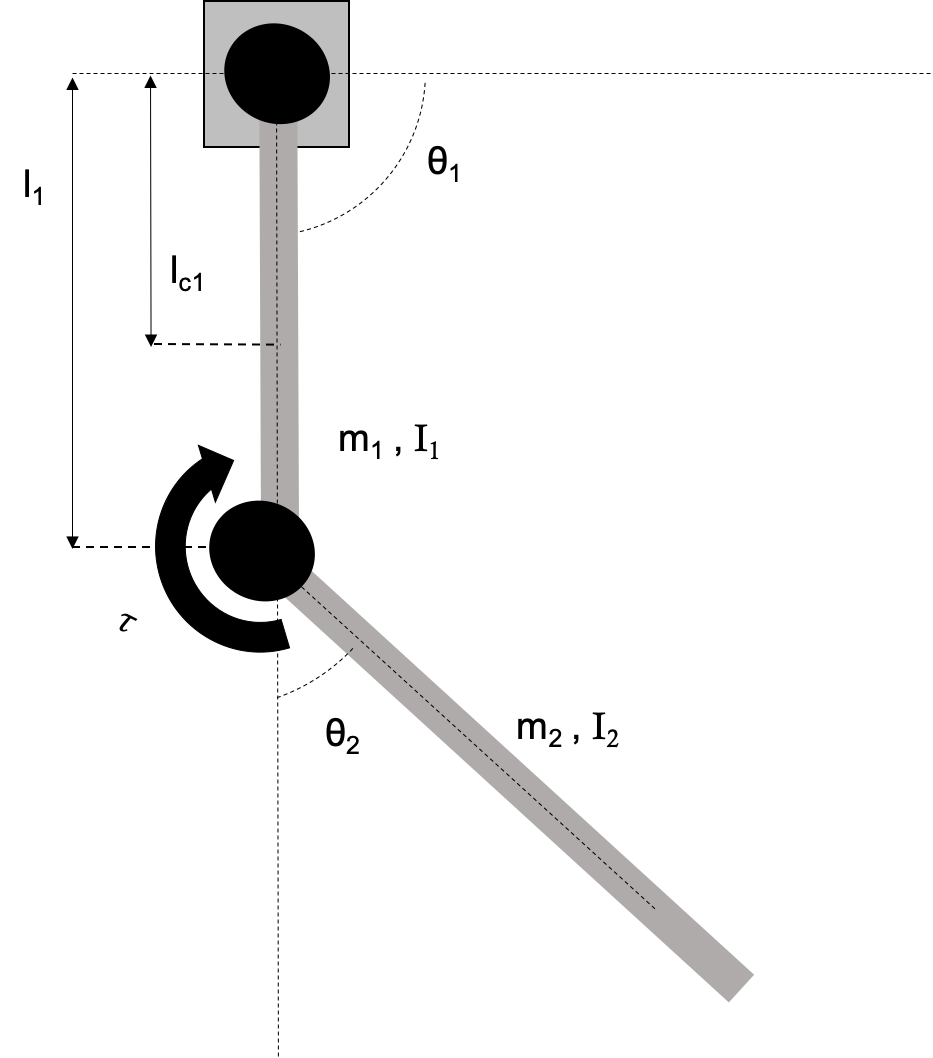
\includegraphics[scale=.25]{acrobot.png}
  \caption{Diagram for the acrobot system, $l_{c*}$ denote the center of mass for each link. $l_{2}, l_{c2}$ follow as $l_{1}, l_{c1}$}
  \label{fig:acrobot}
\end{figure}


The state of this system is $s = [\theta_{1}, \theta_{2}, \dot \theta_{1}, \dot \theta_{2}]$

The goal we wish to achieve is to take this system from any random initial state, to the upright state $gs = [\pi/2, 0, 0, 0]$, which we will refer to as the goal state. 

We implement the system in python, the dynamics are implemented using Euler integration with a time-step of .01s. We experimented with smaller timesteps and higher order integrators, generally we found these made the balancing task easier, but made the wall clock time for the learning much slower.  The reward signal is $r_{t} = l_{1}\sin(\theta_1{1}) + l_{2} \sin(\theta_{1} + \theta_{2}$, following the popular Acrobot-v1 environment \cite{baselines}, and we found empirically that this reward signal actually led to the same outcomes as the more obvious distance in state space. 


The balancing controller is a linear quadratic regulator $C: O \rightarrow U$  about the acrobot's unstable equilibrium. We use the LQR designed by sponge \cite{spong_swing_1994}:

Using 

\[ Q = \begin{pmatrix} 1000 & -500 & 0 & 0 \\ -500 & 1000 & 0 & 0 \\ 0 & 0 & 1000 & -500 \\ 0 & 0 & -500 & 1000\end{pmatrix}, R = \begin{pmatrix} .5 \end{pmatrix}
\]

The resulting control law is: 
\[ u = -Ks \]

with 

\[ K = [-1649.8,  -460.2,  -716.1,  -278.2] \] 

\subsection{Soft Actor Critic}

% policy = $\pi_{\theta}$ \\
% gate   = $G_{\gamma}$ \\
% value = $V_{\phi}$ \\
% target value = ${V}_{\overline{\phi}}$ \\
% Q1 = $Q_{\rho_{1}}$ \\
% Q2 = $Q_{\rho_{2}}$ \\


Soft actor critic \cite{haarnoja_soft_2018} is an entropy regularized reinforcement learning algorithm.% To do the learning we introduce some more neural networks. The %Value function, $V_{\phi}$, which in the entropy regularized setting also includes an entropy bonus such that: 


%\[ V^{\pi}(s) = \mathbb{E}\left[ \sum_{t=0}^{\infty}\gamma^{t}\bigg(R_{t} + \alpha H(\pi(\cdot|s_{t}))\bigg)  \bigg\rvert s_{0} = s\right] \]

%We are also going to learn a Q function which satisfies:

%\[ Q^{\pi}(s,a) = \mathbb{E}\left[ \sum_{t=0}^{\infty}\gamma^{t}\bigg(R_{t}+ \alpha \sum_{t=1}^{\infty} \gamma^{t} H(\pi(\cdot|s_{t}))\bigg)  \bigg\rvert s_{0} = s, a_{0} = a\right] \]


We have a few losses to take care of here:
For the Q fcn:

\begin{dmath} L^{Q} = \mathbb{E}_{s_{t}, a_{t} \sim D}\left[\frac{1}{2}\left( Q_{\rho}(s_{t},a_{t}) - \hat{Q}(s_{t}, a_{t}) \right) ^{2}  \right] \end{dmath}
where
\begin{dmath} \hat{Q}(s_{t}, a_{t}) = r(s_{t}, a_{t}) + \gamma\mathbb{E}_{s_{t+1}}\left[V_{\overline{\phi}}(s_{t+1} ) \right]  \end{dmath}

For the policy network we have:

\begin{dmath} L^{\pi} = \mathbb{E}_{s_{t} \sim D} \left[\infdiv{\pi_{\theta}(\cdot  | s_{t})}{\exp[Q_{\rho}(s_{t}, \cdot)]} \right]  \end{dmath}

To minimize this we make use of a reparameterization trick, that is we take our action as $a_{t} = f_{\theta}(\epsilon_{t}, s_{t})$ where $\epsilon_{t}$ is drawn from $N(0,1)$. This allows us to rewrite $L^{\phi}$ as:


\begin{dmath} L^{\pi} = \mathbb{E}_{s_{t} \sim D, \epsilon_{t} \sim N(0,1)}\left[ \log \pi_{\theta}(f_{\theta}(\epsilon_{t}, s_{t}) | s_{t}) - Q_{\rho}(s_{t}, f_{\theta}(\epsilon_{t}, s_{t}) \right]\end{dmath}


\begin{dmath}L^{\text{value}} = 
\mathop{\mathbb{E}}_{s_{t} \sim D} \left[ \frac{1}{2} \left( V_{\phi}(s_{t}) - \mathbb{E}_{a_{t} \sim \pi_{\theta}} \left[Q_{\rho}(s_{t}, a_{t}) - log \pi_{\theta}(a_{t} | s_{t}) \right] \right)^{2}  \right] \end{dmath} 

This can then be approximated with a clever trick explained in the original paper(!!!) include this or is it a detail we don't need.

With these losses, we can move on to describing the algorithm. Our algorithm starts by doing policy roll outs, recording the state, action, reward, and the active controller at each time step. It stores these experiences in the replay buffer. After enough trials have been run, we run our update step. To this we sample from the replay buffer, and use these sampled states to compute the losses above. We then run n steps of Adam \cite{kingma_adam:_2014} to update our network weights, copy our weights to our target network (which I haven't even talked about) and repeat. 



\section{Switched Soft Actor Critic}

Our primary contribution is to extend SAC in two key ways. 

The first is by modifying the replay buffer $D$. We do this by constructing $D$ from two separate buffers, $D_{n}$ and $D_{r}$. Only roll outs that ended in a successful balance (according to that criteria we discussed above). The other buffer stores all trials, the same as the unmodified replay buffer. Whenever we draw experience from $D$, with probability p we sample from $D_{n}$, and with probability (1-p) we sample from $D_{r}$. We found this to be essential for learning, as even with the LQR and a decent gating function in place, the swingup controller finds the basin of attraction only in a tiny minority of trials. Without the second buffer to hold on to these valuable rollouts we keep learning from rollouts that miss the basin of attraction, and eventually adopt a policy that never visits these states again. 


The second is adding a hand designed LQR to the system, and learning when to switch to this controller . We learn the basin of attraction for the regulator by framing it as a classification problem, our neural network takes as input the current state, and outputs a class prediction between 0-1. A one implying that the LQR is able to stabilize the system, and a zero implying that it cannot. To gather data, we sample a random initial condition, do a policy roll out using the LQR, and record if the controller was successful or not. The success criteria is defined as a trial that has been in the goal state for some amount of time for at least b time steps at the end of training. "Success" here is defined as being withing $\epsilon_{thr}$ of the goal state for at least b time steps at the end of the episode:


\begin{dmath} \norm{s_{t} - gs } < \epsilon_{thr} \quad \forall t \in \{N-b, ...,  N \} \end{dmath}


where N is the length of each episode. To train the gating network we minimize the binary cross entropy loss:


\begin{dmath}L^{\text{G}} =  \mathop{\mathbb{E}}_{\gamma} -\left[ c y_{i}\log(G_{\gamma}(s_{i})) + (1 - y_{i})\log(1 - G_{\gamma}(s_{i})) \right]\end{dmath} 

Where $p$ is a class weight for positive examples, we set $p = \frac{n_{t}}{n_{s}}w $ where $n_{t}$ is the total number of samples, $n_{p}$ is the number of positive examples, and $w$ is a manually chosen weighting parameter to encourage learning a conservative region of attraction. We found that the learned basin was very sensitive to this parameter, a value of .01 empirically works well.


% \begin{algorithm}
% \caption{Warm Start Gate Data Generation}\label{euclid}
% \begin{algorithmic}[1]
% \State Initialize network weights $\gamma$ 
% \For {$i \in \{1, ..., N_{d}\} $}
% \State  sample initial state $s_{0}$ from observation space
% \If {$s_{i} \in B$}
% \State    $y_{i} = 0$
% \Else
% \State    $y_{i} = 1$
% \EndIf
% \EndFor
% \State set $\alpha(0) = 1$, and $\alpha(1) = \frac{\text{sum(y)}}{\text{len(y}}$
% \State update $G_{\gamma}$ with $n_{w}$ steps of Adam to minimize $L^{ws}$
% \end{algorithmic}
% \end{algorithm}

% policy = $\pi_{\theta}$ \\
% gate   = $G_{\gamma}$ \\
% value = $V_{\phi}$ \\
% target value = ${V}_{\overline{\phi}}$ \\
% Q1 = $Q_{\rho_{1}}$ \\
% Q2 = $Q_{\rho_{2}}$ \\

\begin{algorithm}
\caption{Do-Rollout($G_{\gamma}, \pi_{\theta}$, K)}
\begin{algorithmic}[1]
\State $S = R = A = P = R \{\}$
\State  Reset environment, collect $s_{0}$
\For    {$t \in \{0, ..., T\} $}
\State  $p_{t} = hyst(G_{\gamma}(s_{t}))$ 
\If {$(p_{t}) == 1$}
\State    $a_{t} = -Ks_{t}$
\Else
\State   Sample $\epsilon_{t}$ from $N(0, 1)$
\State   $a_{t} = \beta\tanh[\mu_{\theta}(s_{t}) + \sigma_{\theta}(s_{t})*\epsilon_{t}]$ 
\EndIf
\State   Take one step using $a_{t}$,  collect $\{s_{t+1}, r_{t}\}$
\State   $S = S \bigcup s_{t}$, $R = R \bigcup r_{t}$
\State   $A = A \bigcup a_{t}$,  $P = P \bigcup p_{t}$
\EndFor
\State \bf{return} $S,S',A,P$
\end{algorithmic}
\end{algorithm}


\begin{algorithm}
\caption{Switched Soft Actor Critic}\label{euclid}
\begin{algorithmic}[1]
\State Initialize network weights $\theta ,\phi, \gamma, \rho_{1}, \rho_{2}$ randomly
\State set $\overline \phi = \phi$
\For  {$n \in \{0, ..., N_{e}\} $}
\State $S,R,A,P = \text{Do-Rollout}(G_{\gamma}, \pi_{\theta}, K)$
\State Store P in $D_{p}$
\If {$T(S')$}
\State Store $S,R,A$ in $D_{n}$
\Else
\State Store $S,R,A$ in $D_{r}$
\EndIf
\If {Time to update policy}
\State sample $S^{r}, A^{r}, R^{r}$ from $D$
\State $Q^{targ} = R + \gamma V_{\overline{\phi}}(S)$
\State $Q^{min} = \min(Q_{\rho_{1}}(S,A), Q_{\rho_{2}}(S,A))$
\State $V^{targ} = Q^{min} - \alpha*H(\pi_{\theta} (A|S))$
\State Run one step of Adam on $L^{Q}(\rho)$
\State Run one step of Adam on $L^{\pi}(\theta)$
\State Run one step of Adam on $L^{V}(\phi)$
\State   $\overline \phi =  q \overline \phi + (1-q)\phi$
\EndIf
\If {Time to update gate}
\State Run g steps of Adam on $L^{G}$(\phi)
\EndFor
\end{algorithmic}
\end{algorithm}

\section{Results}

\subsection{Training} 
We trained the SSAC for 1e6 timesteps, before that we trained the gate using 1e6 timesteps, so 2e6 steps to train the policy. Hyperparameters were selected by picking the best performing values from a manual search, which are reported in the appendix.

Figure \ref{fig:switched_reward} shows the reward curve for the switched proximal policy optimization. You can clearly see the large gain in reward that is obtained when the switching network is engaged after the warm start period.

 \begin{figure}[h]
\centering
  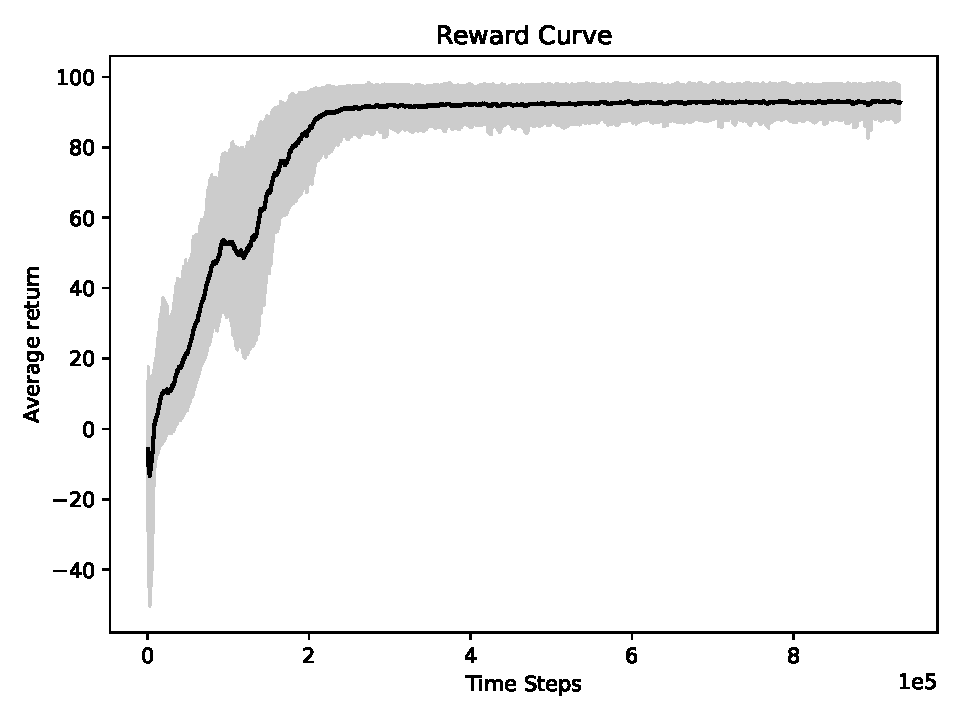
\includegraphics[scale=.5]{reward_curve.pdf}
  \caption{Reward curve for the switched PPO. Black line is the smoothed average of episode reward, averages over four random seeds. The shaded grey area indicates the best and worst rewards at each epoch across the four seeds. A reward of 2000 would imply the system was in the goal state for the entire episode}
  \label{fig:switched_reward}
\end{figure}

In addition to training on our own version of SAC and Switched SAC we also examined the performance of several algorithms written by OpenAI and cleaned up by the community \cite{stable_baselines}. We examine PPO and TRPO, two popular trust region methods. A2C was included to compare to a non trust region, modern policy gradient algorithm. We also include TD3, which is very similar to the DDPG and D4PG, which have been shown in the literature to do well on the acrobot and cartpole problems \cite{lillicrap_continuous_2015} \cite{deepmindcontrolsuite2018}. 
Stable baselines includes hyperparameters that were allegorically tuned for each environment. For algorithms where parameters for Acrobot-v1  were available we chose those, some algorithms were missing Tuned Acrobot-v1 examples, and for those we used parameters for Pendulum-v0, simply because it is another continuous, low dimensional task. Note we don't expect the hyper-parameters to make or break the performance per say, only effect how fast learning occurs. Reported rewards are averaged over 4 random seeds. Every algorithm makes 2e6 interactions with the environment. Also note that this project was largely inspuired by spending a large amount of time manually tuning these parameters to work on this task



\begin{center}
\begin{tabu}{| X[l] | X[l] |}
\hline
Algorithm (implementation) & Mean Reward $\pm$ Standard Deviation\\
 \hline
 SSAC (Ours) & \bf{92.12 $\pm$ 2.35}  \\ 
 \hline
 PPO (Baselines) &  0.43 $\pm$ 8.89 \\ 
 \hline
 TD3 (Baselines)  & 78.67  $\pm$ 61.85 \\
 \hline
 TRPO (Baselines) &  17.63 $\pm$ 3.39 \\
 \hline
 A2C (Baseline)   & 2.57 $\pm$ 3.63 \\
 \hline
\end{tabu}
\label{table:results}
\end{center}

As we can see, for this environment, with the number of steps we have allotted, our approach outperforms all the algorithms we tried, with Td3 making it the closest to our performance. This is a necessarily flawed comparison. These algorithms are meant to be general purpose, so it is unfair to compare them to something designed for a particular problem. But that is part of the point we are making, that adding just a small amount of domain knowledge can improve performance dramatically.

\subsection{Analyzing performance}

To qualitatively evaluate the performance of our learned agent we examine the behavior during individual episodes. During training we treat the output of the action and gating network as the means of a probability distribution, which are then sampled from. However this random sampling is to encourage exploration, and to help obtain robust policy, at test time we are free to pick only the most likely controller and action pair. This adds the advantage of giving us a deterministic controller, which makes evaluation a lot clearer. And again, we think it's remarkable that these algorithms, without much tuning, can solve much harder problems!

 \begin{figure}[h!]
\centering
  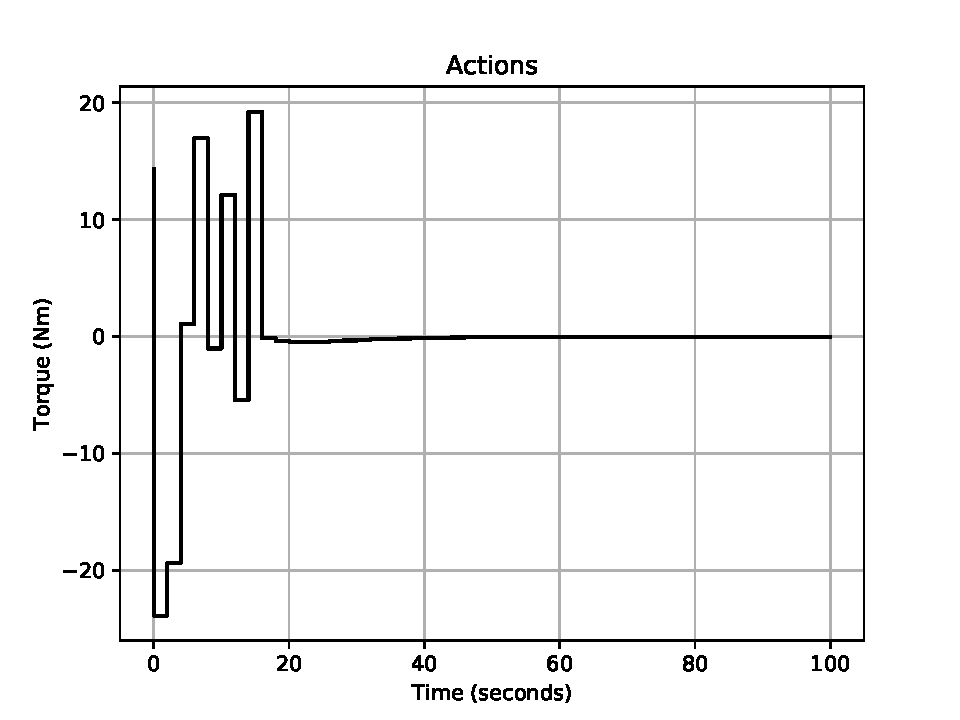
\includegraphics[scale=.5]{act_hist.pdf}
  \caption{Torque exerted during the sampled episode !! this is a placeholder}
  \label{fig:act}
\end{figure}

\begin{figure}[h!]
\centering
  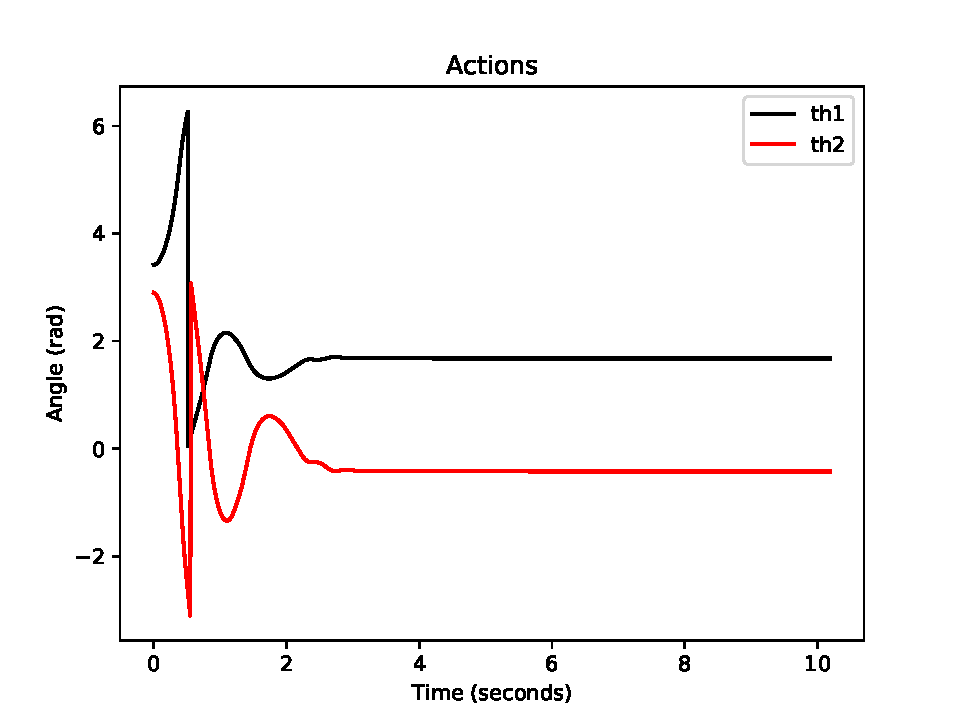
\includegraphics[scale=.5]{obs_hist.pdf}
  \caption{Observations during an episode !! this is a placeholder}
  \label{fig:act}
\end{figure}


We can see in figure \ref{fig:act} the actions selected by the controller. It is clear that the agent has learned a very aggressive swing-up policy, which the LQR is able to grab and hold onto. This makes sense as our reward function does not include penalties on actions or velocities, so the optimal action is to swing up the pole as fast as is possible without causing the LQR to fail to stabilize the system.  

Figure \ref{fig:rew} shows the reward during the episode. Recall that our reward function was merely the height of the acrobots second link, which makes it easy to interpret, and we can use this as a proxy for the rest of our state variables.   


We also display the mean outputted by the gate function during the episode, we can see that the agent learned to to use a very short swing-up phase to maximize it's reward. 

Because our system is relatively low dimensional, we can attempt to visualize the outputs of our networks. We found that examining the output of the gating network provided insight into what was learned during training. We found this network did not vary much with the velocity variables, so we show the output for a cross section of the state space, as $\theta_{1}$ and $\theta_{2}$ vary across their range. Figure \ref{fig:gate_pre} shows the gate mapping after the warm start but before training, and figure \ref{fig:gate} shows the value after the switched training. 

\begin{figure}[h]
\centering
  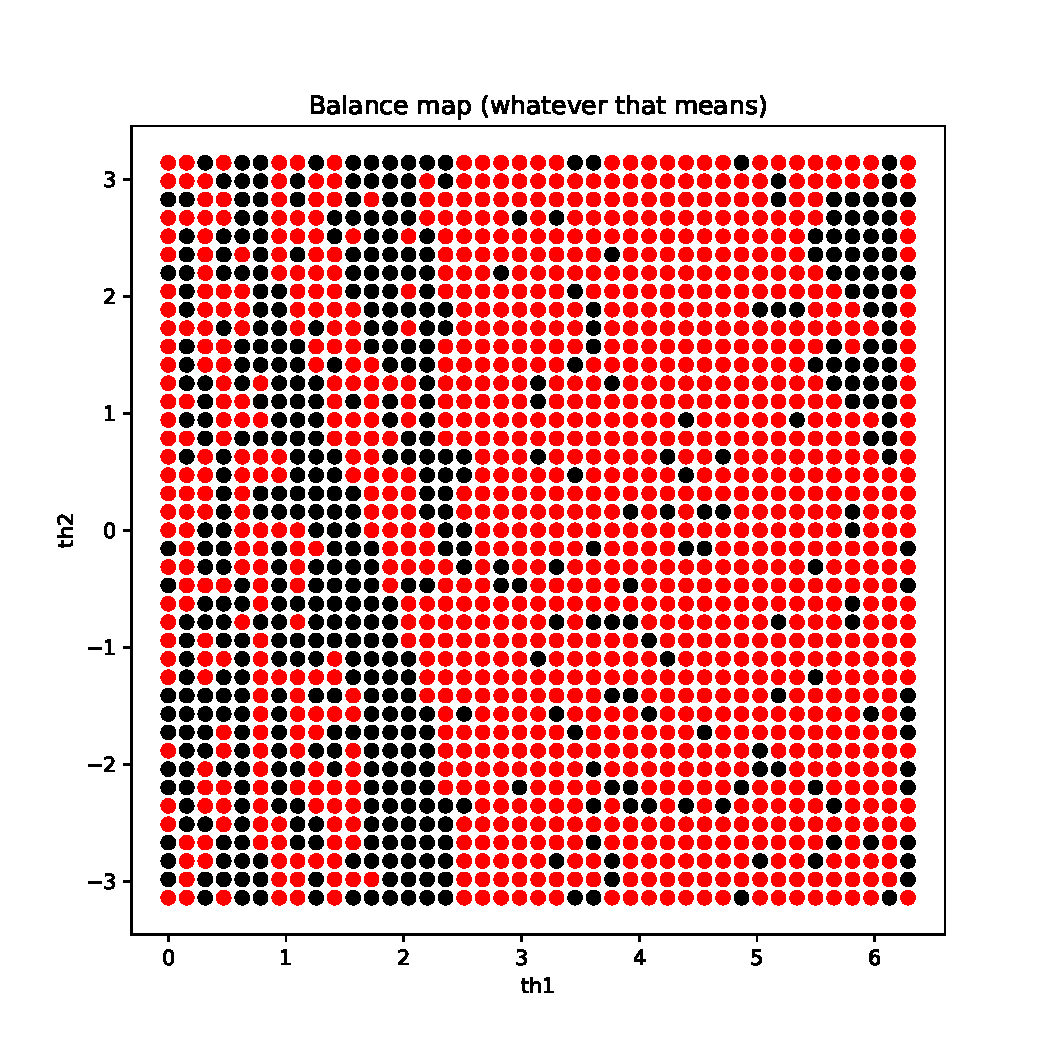
\includegraphics[scale=.4]{th_map.pdf}
  \caption{!! Not convinced this is the moves}
  \label{fig:gate_pre}
\end{figure}

\begin{figure}[h]
\centering
  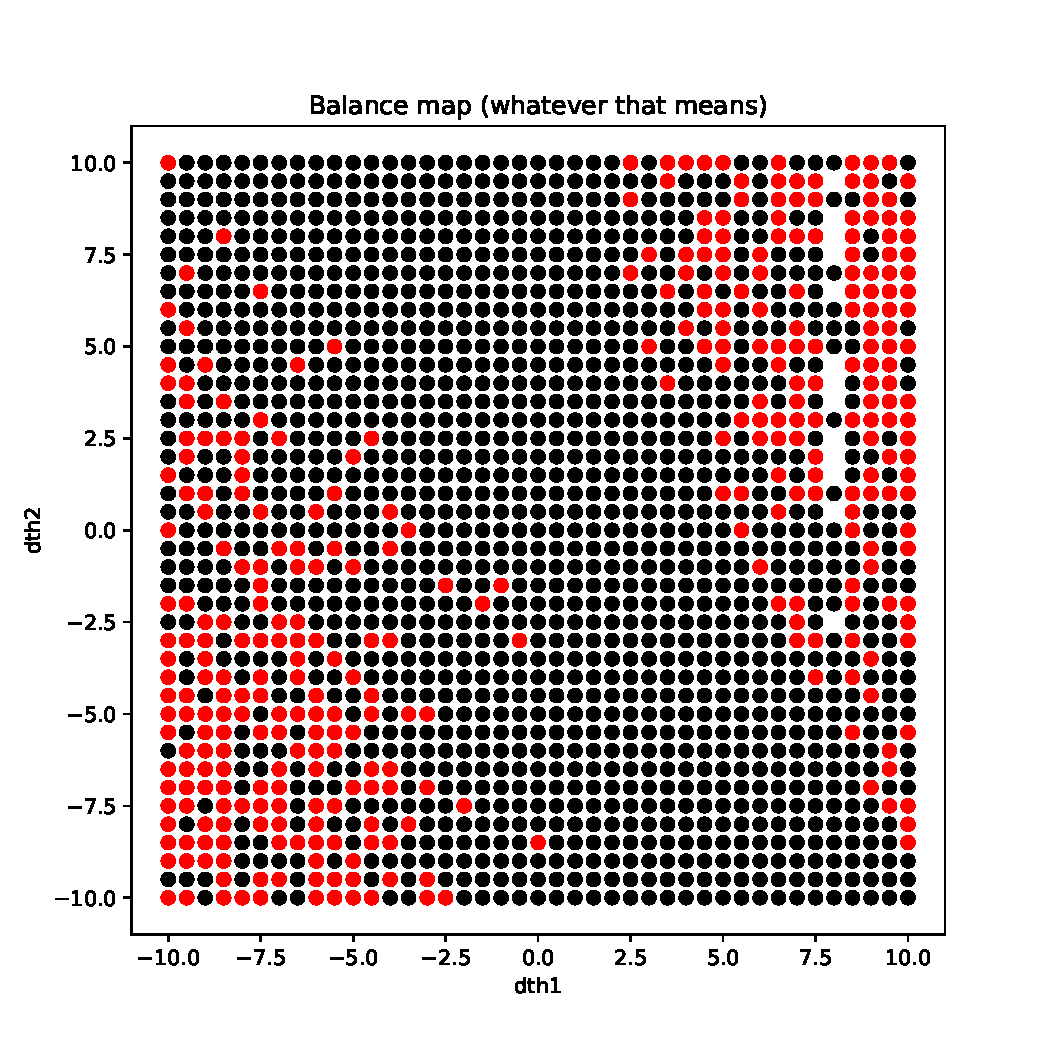
\includegraphics[scale=.4]{dth_map.pdf}
  \caption{!! Not convinced this is the moves}
  \label{fig:gate}
\end{figure}


The initial state is at the bottom center of this picture, we can see that the algorithm learned that the estimate we gave it for when to use the LQR turned out to be conservative for the states it was seeing during training. And we see this region expands significantly after training.



\section{CONCLUSIONS}

We have presented a novel control design methodology that allows engineers to leverage their domain knowledge, while also reaping many of the benefits from recent advances in deep reinforcement learning. In our case study we constructed a policy to swing up and balance an acrobot while only needing to manually design a linear controller for the balancing task. We believe this method of control will be straightforward to apply to the double or triple cartpole problems, which to our knowledge no model free algorithm is reported as solving. We also think that this general methodology can be extended to more complex problems, such as legged locomotion. In that case the linear controller here could be a nominal walking controller obtained via trajectory optimization, and the learned controller could be a recovery controller to return to the basin of attraction of this nominal controller. 
%%%%%%%%%%%%%%%%%%%%%%%%%%%%%%%%%%%%%%%%%%%%%%%%%%%%%%%%%%%%%%%%%%%%%%%%%%%%%%%%



%%%%%%%%%%%%%%%%%%%%%%%%%%%%%%%%%%%%%%%%%%%%%%%%%%%%%%%%%%%%%%%%%%%%%%%%%%%%%%%%

\bibliographystyle{IEEEtran}
\bibliography{IEEEabrv,IEEEexample}

%%%%%%%%%%%%%%%%%%%%%%%%%%%%%%%%%%%%%%%%%%%%%%%%%%%%%%%%%%%%%%%%%%%%%%%%%%%%%%%%
\section*{APPENDIX}

\subsection*{Hyperparameters}

\begin{center}
!!!!

\begin{tabu}{ X[2,l] | X[1,l] }
Hyperparameter & Value \\
 \hline
 Episode Length (N) & 1000  \\ 
 Batch Size (T) & 2048  \\ 
 Initial policy learning rate & 1e-5  \\ 
 Initial value learning rate & 1e-4  \\ 
 Initial gate learning rate & 1e-5  \\ 
 Action variance ($\sigma_{\pi}$) & 2 \\
 Gate variance ($\sigma_{\gamma}$) & .2 \\
 Discount ($\gamma$)   & 1 \\
 GAE parameter ($\lambda$)  & .99 \\
 Clipping parameter $\epsilon$ & .2 \\
 Policy updates per epoch ($n_{p}$) & 10 \\
 Value updates  per epoch ($n_{v}$) & 10\\
 Gate updates   per epoch ($n_{g}$) & 10\\
 \hline
\end{tabu}
\end{center}

\begin{center}
Vanilla PPO
\begin{tabu}{ X[2,l] | X[1,l] }
Hyperparameter & Value \\
 \hline
 Episode Length (N) & 1000  \\ 
 Batch Size (T) & 2048  \\ 
 Intial policy learning rate & 1e-3  \\ 
 Action variance ($\sigma_{\pi}$) & 2 \\
 Discount ($\gamma$)   & 1 \\
 GAE parameter ($\lambda$)  & .99 \\
 Clipping parameter $\epsilon$ & .2 \\
 Policy updates per epoch ($n_{p}$) & 10 \\
 Value updates per epoch ($n_{v}$) & 10\\
 \hline
\end{tabu}
\end{center}

\subsection*{Network Architecture}
The policy, value, and Q networks are all made of four fully connected layers, with 32 hidden nodes and Relu activations. The gate network is composed of two hidden layers with 32 nodes each, also with Relu activations, the last output is fed through a sigmoid to keep the result between 0-1.


\subsection{Linear Quadratic Regulator Design}


%%%%%%%%%%%%%%%%%%%%%%%%%%%%%%%%%%%%%%%%%%%%%%%%%%%%%%%%%%%%%%%%%%%%%%%%%%%%%%%%


\addtolength{\textheight}{-12cm}   % This command serves to balance the column lengths
                                  % on the last page of the document manually. It shortens
                                  % the textheight of the last page by a suitable amount.
                                  % This command does not take effect until the next page
                                  % so it should come on the page before the last. Make
                                  % sure that you do not shorten the textheight too much.


\end{document}
